\section{System Overview}
%
\begin{figure}[bt]
  \begin{center}
%    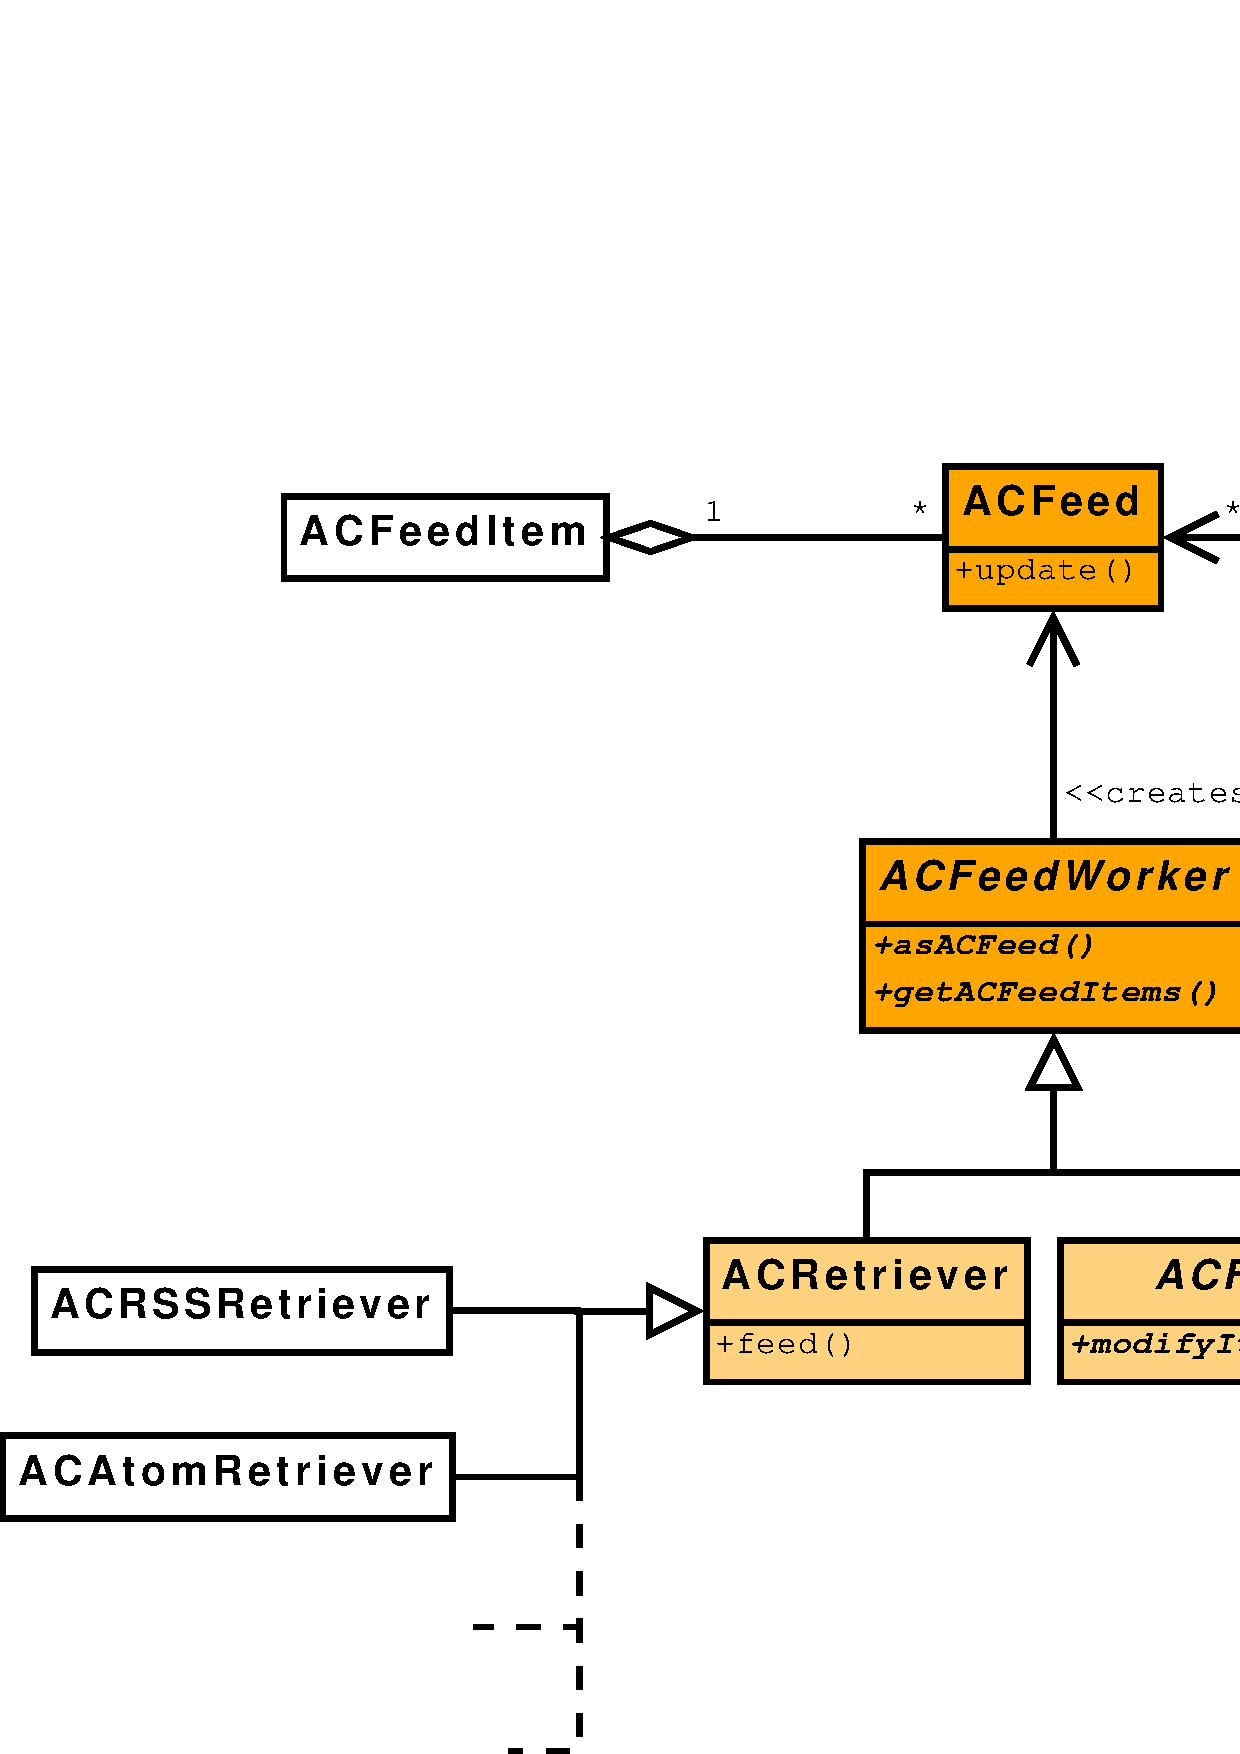
\includegraphics[width=0.9\linewidth]{images/system.png}
  \end{center}
  \caption{The complete system overview}
  \label{fig:system}
\end{figure}
%
\subsection{Interactions and Responsibilites}
\subsubsection{Themes and External Resources} ~\\
The FBTheme class is implemented as flyweight, holding references to previously 
created instances of a particular theme. If a requested theme type is not yet 
held in the list of instances, the class calls a builder class, 
FBThemeBuilder~\ref{fig:system}(1), to parse the requested theme's XML file, 
load the images and then return a fresh instance of the theme. Additionally, 
each theme contains an FBImageLibrary. The image library is just a simple 
wrapper around an IdentityDictionary to ease filling it with Forms. 
FBTheme and FBImageLibrary also support scaling to adjust to any screen 
size (without accounting for neccessary interpolation).
The FBImageLibrary is filled prior to starting the actual game, so 
that all external resources are cached. A lazily initialized image 
library would have resulted in slow disk I/O during
run-time.
\subsubsection{Rewarding the Players} ~\\
FBRewardStrategies are supporting classes which add rewarding behaviour 
to the game logic
~(Fig.\ref{fig:system}(2)). Its specializations 
implement different strategies to
reward the players for good gaming. Good gaming is measured by the 
number of balls falling, if more are falling at the same time, more 
reward points are gained.
The reward strategies have to implement a method
rewardPlayer:for:~\ref{lst:reward}.\\
In single player mode, a FBHighscoreReward
adds a simple highscore to the screen (responsible for adding the 
score visual is also the strategy itself) and for any number of 
reward points reported by the FBPlayfield, score points are accumulated.
%
\begin{lstlisting}[float,label=lst:reward,caption=The Highscore Calculation Method]
FBHighscoreReward>>rewardPlayer: aPlayer for: anAchievmentScalar
    "I reward a single player with an exponentially 
rising rate of points" 

    self score:
         self score + (anAchievmentScalar raisedTo: 2)
    \end{lstlisting}
%
In multiplayer mode, the strategie only rewards, if the player eliminates 
more than three balls from the field with a single shot. If that happens, 
a number of balls half as great is distributed among the other players,
and shot randomly in any direction. This happens via a call to 
the playfields which have to shoot random balls, since FBRewardStretegies
hold a collection referring to all playfields.
%
\subsubsection{Playfield Morphs} ~\\
As aforementioned, FBPlayfield is responsible for creating its own 
contents~\ref{fig:system}(3). Such content displays a cannon, a 
player avatar , messages for the user and numerous coloured balls. 
Each of these serves only a single, limited purpose, with FBPlayer 
and FBMessage merely wrapping different types of graphical response.
The cannon is the entity that reacts to the user's input, panning 
left and right and sending balls off into the field. However, it 
is controlled entirely by the playfield and does not act itself.

The FBBall is an exception to this simplicity. 
\begin{description}
  \item[First]
    	it has to look 
	differently, showing different colors in our themes. 
  \item[Secondly]
    	a Ball has different stages in its lifetime, being 
	loaded into the cannon, then flying, hanging from the 
	ceiling (or, indeed, from other balls) and finally falling 
	and vanishing.
  \item[Finally]
    	a Ball needs to collide with the playfield boundaries and 
	other balls in the field.
\end{description}
Thus its implementation is a bit larger, as it implements the FBCollider 
interface, utilizes different ``states'' to act on in its step method and 
and also draws itself from a collection of images.
%
\subsection{FBCollisionMap}
% \ref{sec:collision}
Collision detection is handled by one collision map per playfield. This collision
map is an instance of FBCollision. A collision is detected a posteriori, meaning
that the ball first moves to the next position and  than checks whether it collides
with some other object. However, this is not strictly necessary and not reflected in
the implementation of the collision map. Any object may ask the collision map wheter
a collision is happening at a given point on the map and may react accordingly. There
are two kinds of collision: One where a ball usualy should get stuck and one where it
should bounce of. As can be seen in Listing \ref{lst:ifBounceOff}, the API call wraps
around doYouGetStuckAt: and doYouBounceOff: - checking in that order, since if a ``stuck
collision'' should occure, it has a higher priority than a ``bounce of collision''.

\begin{figure}
  \begin{center}
    \begin{lstlisting}
at:aPoint ifBounceOff:bounceOffBlock ifGetStuck:getStuckBlock
	
	(self doYouGetStuckAt: aPoint)
		ifTrue: [getStuckBlock value]
		ifFalse: [ (self doYouBounceOff: aPoint)
			ifTrue: bounceOffBlock ]
    \end{lstlisting}
  \end{center}
  \caption{API method for detecting collision}
  \label{lst:ifBounceOff}
\end{figure}
%
\subsection{FBSweeper}
As discussed in \ref{sec:garbage}, the first design planned for every Ball to keep track of all Objects it holds on to and all Objects that hold on to it. When an Object falls down, it informs the objects that hold on to it, via the Squeak built-in event mechanism~\cite{website:squeakwikiObserver}, that they lost one Holder. When an Object has lost its last Holder, it should itself fall down and inform all objects that hold on to it that it is gone.
This approach had several drawbacks. First, the logic for this falling down was distributed over the CollisionMap, Ball and Ball classes.
Second, every Ball observed the Balls next to it. When a Ball was removed from the structure, the observing Balls removed it from their lists of holders. In the event that a Ball had no holders, it fell down, thereby invoking events on its observing neighbours.
This resulted in a control flow that was hard to understand, as the information of the removal of a Ball was propagated to the other Balls implicitly through events and not explicitly through messages.
Third, reference-counting garbage collectors have a well-known problem with cyclic references. 

In order to separate the concern of letting-balls-fall-down the from the Rest of the Game logic, the FBSweeper was introduced.

Like a mark-and-sweep garbage collector, the sweeper traverses the Balls in the Playfield and marks every Ball it can reach, beginning with the balls that stick to the top of the FBPlayfield.  In the beginning, all Balls are considered for collection and thus contained in the gcCollect set. Marking happens by removing a FBBall from the set. When a Ball is reachable and has not yet been marked, it is marked and its neighbours, determined through the collision map, are considered reachable. This is repeated until all reachable Balls have been marked, then all remaining Balls are unreachable and can be removed.
The Balls are traversed breadth-first.

\begin{lstlisting}[language=Smalltalk, label=lst:sweep, caption= mark-and-sweep ball collector, float]
FBSweeper>>sweep: aCollisionMap
    "Sweep balls that do not hang on anything 
off the playfield"
    |gcLive gcCollect|
    gcCollect := gcArena copy.
    gcLive := gcRoots copy.
    [gcLive isEmpty] 
        whileFalse:[
            gcLive copy do: [:eachLiveBall|
            gcLive remove: eachLiveBall.
            (gcCollect includes: eachLiveBall) 
	        ifTrue:[
                    gcCollect remove: eachLiveBall.
                    gcLive addAll:
                        (aCollisionMap 
		            holdersFor: eachLiveBall center)
        ]]].
    gcCollect do:[:deadBall | deadBall fall].
\end{lstlisting}


